%& -aux-directory=/tmp
% sorgt  dafuer dass aux files sonstwohin kommen -output-directory=C:/pdfout
\documentclass[10pt,a4paper, fleqn]{article}
% twocol class oder so geht auch
% fleqn macht align formeln nach lings
\usepackage[utf8]{inputenc}
\usepackage{hyperref}
\hypersetup{linktocpage}
%\usepackage[ngerman]{babel}
\usepackage{amsmath} % xrightarrow, ...
\usepackage{cite}
\usepackage{units} % nicefrac
\usepackage{datetime} % fuer Uhrzeit im \date
%\usepackage{wrapfig} % bilder rechts
\usepackage{caption} % fuer subcaption
%\usepackage{subcaption} % subfigures
\usepackage{graphicx} % Bilder allgemein einbinden
%\usepackage{tabularx} % Tabellen
\usepackage{lastpage} % Anzahl Seiten
\usepackage{multicol} % zweispaltige Titelseite
\usepackage{a4wide} % bessere Papiernutzung
\usepackage{fancyhdr} % Header/Footer
%\pagestyle{fancy} % Kopf/Fussbereich der Seiten
\usepackage{amssymb} % therefore = dreieckdots
\usepackage{array} % tables
\usepackage{booktabs} % better tables

% zweispaltiger Text
\usepackage{multicol}
%\setlength{\columnseprule}{0.4pt}

% Ueberschriften kleiner 	
%\usepackage{titlesec}
%\titleformat{\section}{\large\bfseries}{\thesection}{1em}{}
%\titlespacing{\paragraph}{%
%  0pt}{%              left margin
%  0.5\baselineskip}{% space before (vertical)
%  1em}%               space after (horizontal)
%%\titlespacing{\section}{0pt}{0.2\baselineskip}{0.1\baselineskip}
%\titlespacing{\align}{0pt}{0.2\baselineskip}{0.1\baselineskip}
%\titlespacing{\equation}{0pt}{0.2\baselineskip}{0.1\baselineskip}

% abgefahrenes highlighting von formeln
\usepackage{xcolor}
% klappt net, was einfacheres:
\newcommand{\highlight}[1]{%
  \colorbox{green!30}{$\displaystyle#1$}}

% Kopfzeile/Fusszeile mit fancy
%\fancyhead{}
%\fancyfoot{}
%\fancyfoot[FL]{\slshape F-Praktikum, Supraleiter}
%\fancyfoot[FR]{\slshape Page \thepage {} / \pageref*{LastPage}}
%\renewcommand{\headrulewidth}{0 pt}

% Bibliography
\bibliographystyle{ieeetr}

% Farben (werden derzeit nur in hypersetup verwendet)
\usepackage{color}
\definecolor{darkblue}{rgb}{0,0,.6}
\definecolor{darkred}{rgb}{.1,0,0}
\definecolor{darkgreen}{rgb}{0,.5,0}

% Schriften
% Palatino for rm and math | Helvetica for ss | Courier for tt
\usepackage{mathpazo} % math & rm
\linespread{1.05}        % Palatino needs more leading (space between lines)
\usepackage[scaled]{helvet} % ss
\usepackage{courier} % tt
\normalfont
\usepackage[T1]{fontenc}

% Hyperref aufsetzen
\hypersetup{
    pdftitle={Master Physik bei Nicolini, Calc writeup},
    pdfauthor={Sven Köppel},
    pdfsubject={master},
    pdfkeywords={physik} {master} {uni} {frankfurt} {fias},
    colorlinks=true,        % test: stat gerahmten Links
    linkcolor=red,          % color of internal links
    citecolor=darkgreen,    % color of links to bibliography
    filecolor=darkred,      % color of file links
    urlcolor=cyan           % color of external links
}

% Allgemeine Meta-Daten, derzeit ungenutzt
\title{\vspace{-9ex} Calc10 \vspace{-1ex}} % vertikalen platz weg...
\author{\small %
\href{https://itp.uni-frankfurt.de/~koeppel}{Sven Köppel} \\
\small \texttt{koeppel@fias.uni-frankfurt.de}}
\date{\small Generation date: \today, \currenttime}


\begin{document}
\maketitle

% abkuerzungen:
\renewcommand{\d}{\mathrm{d}}
\newcommand{\dd}[2]{\frac{\mathrm{d} #1}{\mathrm{d} #2}}
\newcommand{\pp}[2]{\frac{\partial #1}{\partial #2}}
\renewcommand{\L}{L_P}
\newcommand{\pr}{p_r}
\newcommand{\psenk}{p_\perp}
\newcommand{\ebenso}{\biggl( ~ \therefore ~ \biggr) }
\newcommand{\metrik}[1]{\d s^2 = \left( #1 \right) \d t^2 \left( #1 \right)^{-1} \d r^2 + r^2 \d \Omega_{D-2}^2 }
\newcommand{\winkel}{r^2 \d \Omega^2}
\newcommand{\dann}{$\rightarrow~$}
\newcommand{\CA}{ {\cal A}}
\newcommand{\C}[1]{ {\cal #1}}
\newcommand{\mn}{_{\mu\nu}}

\begin{multicols}{2}
Calc10 ties up Calc8, calculating the Propagator and modified Einstein Equations.

\columnbreak
\tableofcontents
\end{multicols}

\section{The modified Action}
The aim of this section is to motivate potential $V(r) \propto \frac {h(r)}{r^{1+n}}$ in the metric $g_{00} = 1 - V(r)$ not only as the result of a modified density $\rho = \frac M{\Omega} \delta(r) \to \frac M{\Omega} \dd {h(r)}r$ but also by modified Einstein equations, a modified Action, a modified mass or gravitational constant term. That is, the step $\delta(r) \to \dd{h(r)}r$ shall be performed by introducing a more fundamental concept.

This concept looks like a modified delta distribution again: A bilocal distribution

\begin{equation}
\CA^2(x-y) = \CA^2(\square_x) \delta^4(x-y)
\end{equation}

One way to introduce it is smearing the Ricci scalar $R(x)$  [N 02.2012] by

\begin{align}
\C R(x) &= \int \d^4 y \sqrt{-g} \CA^2 (x-y) R(y)
\end{align}

This modifies the Action and the Einstein equations immediately:

\begin{align}
&S = \frac 1{16\pi G} \int \d^4x \sqrt{-g} \C R(x)
&\CA^2(\square) \left( R_{\mu\nu} - \frac {g_{\mu\nu}}2 R \right) = 8\pi G~T_{\mu\nu}
\end{align}

Having $\C T\mn = \CA^{-2}(\square) T\mn$ and the Schwarzschild density $\rho_0 = M\delta(\vec x)$, we end up with

\begin{equation}
\C T^0_0 = -M \CA^{-2}(\square) \delta(\vec x)
\end{equation}

Finally, this yields our requirement for matching this formalism to the holographic approach in [Calc 1-10]:

\begin{equation}
M \C A^{-2}(\square) \delta(\vec x) \stackrel{!}{=} \frac M{\Omega_{n+2}} \dd{H(r)}r  \label{eq:Master}
\end{equation}

I want to find profiles $\C A$ that corresponds to my functions $H \in \{ h, h_\alpha\}$ in $n$ dimensions.

\subsection{Operator rewrites and Fourier Transformation}
In [N 02.2012], there is a special choice of the D'Alambert operator, using a length scale $\ell$. This gives the momentum operator $\hat P$ another form than usual:

\begin{align}
\hat P &= - i \hbar \nabla \\
\square &= \ell^2 \nabla^2 \\
\Rightarrow\quad \hat P^2 &= - \square / \ell^2 \label{eq:thep}
\end{align}

\subsubsection{Spherical Fourier transformation in $3+n$ dimensions}
I use the Fourier transformation $\C F$ which is defined in $d$ dimensions ($\vec x \in \mathbb R^d$) as

\begin{align}
\C F\left\{ f \right\}(\vec p) &= \tilde f(\vec p) = \frac 1{(2\pi)^d} \int \d^d x~e^{-i\vec p \cdot \vec x} f(\vec x) \label{eq:Four1} \\
\C F^{-1}\left\{ \tilde f \right\}(\vec x) &= f(\vec x) =   \int d^d p~e^{+i \vec p \cdot \vec x} \tilde f(\vec p) \label{eq:Four2}
\end{align}

The subsequent use is in $d=3+n$ dimensions. If the function $f$ only depends on the radius, $f(\vec x)=f(|\vec  x|)$, then the integrals \ref{eq:Four1} and \ref{eq:Four2} can be transformed to one dimensional integrals. In $d=3$, we obtain

\begin{align}
\hat V(p) &= \int \d^3 r ~e^{-i \vec r \cdot \vec p}~ V(r) = 2\pi \int_{-1}^{+1} \d \cos \theta \int_0^\infty \d r ~r^2 ~e^{-i r p \cos \theta} V(r) \\
&= \frac{2 \pi i}{p} \int_0^\infty \d r ~r ~V(r) \left( e^{-irp} - e^{+irp} \right) \\
&= \frac{2 \pi i}{p} \left[
\int_0^\infty e^{-ipr}~r~V(r)
- \int_{-\infty}^0 e^{-ipr}~(-r)~V(-r)
\right] \\
&= \frac{2\pi i}{p} \int_{-\infty}^\infty \d r ~e^{-irp} ~r ~\left[ V(r) \Theta(r) + V(-r) \Theta(-r) \right] \label{eq:FourNinf}
\end{align}

with $r=|\vec r|$, $p=|\vec p|$.

% Note that this effectively amounts to an one dimensional Fourier transform
%
%\begin{equation}
%\hat v(p) = \int_{-\infty}^\infty \d r ~e^{-irp} ~v(r)
%\end{equation}
%
%with
%
%\begin{equation}
%v(r) = r~\left[ V(r) \Theta(r) + V(-r)\Theta(-r)\right]
%\quad\text{and}\quad
%\hat V(p) = \frac{2\pi i}p \hat v(p)
%\end{equation}

The rewrite made the trick of substituting the $\theta \in [0,\pi]$ angle by the angle between $\vec r$ and $\vec p$ in the scalar product $\vec r \cdot \vec p = |\vec r|~|\vec p| \cos \varphi$, with $\varphi \in [0,\pi]$. This is also possible in higher dimensions. Consider in the spherical spacial coordinates $\vec r = (r,\phi,\theta_1,\dots,\theta_{d-2})$:

\begin{align}
\int \d^d r &= \int_0^\infty \d r ~r^{d-1}
\int_0^{2\pi} \d \phi
\prod_{i=1}^{d-2} \int_0^\pi \d \theta_i \sin^i (\theta_i)
:= \int_0^\infty \d r ~\Omega_{d-1} r^{d-1} \\
&= \frac {\Omega_{d-1}}2 \underbrace{\int_0^\pi \d \theta_1 \sin(\theta_1)}_{=2} \int_0^\infty \d r ~r^{d-1}
\quad\quad
\text{with}
\quad
\Omega_{n+2} = 2 \frac{\pi^\frac{n+3}{2}}{\Gamma\left(\frac{n+3}{2}\right)}
\end{align}

Making the scalar product substitution with only $\theta_1$, one gets

\begin{align}
\tilde V(p) &= \frac {\Omega_{d-1}}{2}
\frac ip  \int_0^\infty
\d r~r^{d-2}~V(r)~\left(e^{-irp} - e^{+irp}\right) \\
&= \frac {\Omega_{n+2}}{2}
\frac ip  \int_0^\infty
\d r~r^{n+1}~V(r)~\left(e^{-irp} - e^{+irp}\right) \label{eq:FinalVpNdim}
\end{align}

When writing the integral in form of (\ref{eq:FourNinf}), the Residual theorem

\begin{equation}
\frac{1}{2\pi\mathrm{i}}\int_\Gamma f=\sum_{a\in D_f}\operatorname{ind}_{\Gamma}(a)\operatorname{Res}_a f
\end{equation}

can be used to solve these integrals.
%
%\subsubsection{Falsche Interpretation}
%Das hier hab ich falsch verstanden, oben ist richtig:
%
%Such an integral rewrite is also possible in higher dimensions, but the angles cannot be integrated out any more, at least not before integrating the radial part, because the Exponential Integral occurs. Consider for $n=1$  the problematical part of the integral:
%
%\begin{equation}
%\int_{-1}^{+1} \d \cos \theta_1
%\int_{-1}^{+1} \d \cos \theta_2
%\int_0^\infty \d r r^3 e^{-i r p \cos \theta_1 \cos \theta_2}
%\end{equation}
%
%After performing the first integral, one cannot proceed. With $\cos \theta_i = c_i$:
%
%\begin{equation}
%\int \d c_1 
%\int \d c_2 ~ e^{c_1 c_2}
%=
%\int \d c_1
%\left[
%\frac {e^{c_1 c_2}}{c_1}
%\right]_A^B
%\approx
%\int \d c_1
%\frac {e^{c_1}}{c_1}
%\end{equation}
%
%$(2+n)$-dimensional integrals can only be handled by first integrating the radial part, then the angles:
%
%\begin{equation}
%\tilde V(p) = 2\pi
%\prod_i^{1+n} \int_{-1}^{+1} \d c_i
%\int_0^\infty \d r ~r^{2+n} ~ f(r) e^{i r p \prod_i c_i}
%\end{equation}

\subsubsection{Operator Eigenvalues}
We also use the so called Schwinger-Representation ([IMN Nov 2013], eq. 21) for operators $\C O$ (actually, I don't know why):

\begin{equation}
(\C O)^\alpha = \frac 1{\Gamma(-\alpha)} \int_0^\infty \d s~ s^{\alpha - 1} e^{-s \C O}
\end{equation}

Furthermore, power series are used to reason why functions of operators can be replaced by functions of the applied operators. E.g.

\begin{align}
\exp x &\approx 1 + x + \frac {x^2}2 + \frac {x^3}6 + \dots \\
\frac 1{1+x} &\approx 1 - x + x^2 - x^3 + \dots
\end{align}

Consider linear operators, especially differential operators $\C O = \dd{}x$. Then consider any infinetly differentiable function $f$ of that differential operator $\dd{}x$. I will switch between the representations $f(\dd{}x)$ and $f(p)$, which does {\it not} denote momentum space, but an evaluation of differentiation. The eigenvalue equation with eigenfunction $e^{\lambda x}$

\begin{equation}
f\left(\dd{}x\right) ~ e^{\lambda x} = f(\lambda) ~ e^{\lambda x}
\end{equation}

makes that replacement feasible. In the next section, this will be used with a semi-Fourier-transform:

\begin{equation}
f\left(\dd{}x\right) ~ \delta(x) = f(p^2) ~ \delta(x)
\end{equation}


\subsection{How to get the $\CA$}
We want to solve eq. (\ref{eq:Master}). This can be done exploiting one dimensional Fourier Transformationations. Consider the Fourier transformation of the Dirac Delta $\delta(x)$,

\begin{align}
&\tilde \delta(p) = \frac 1{2\pi} \int \d x~e^{-ipx} \delta(x) = 1
&\delta(x) = \int \d p~e^{ipx}  \label{eq:Fdelta}
\end{align}

We write both sides of (\ref{eq:Master}) as the reverse Fourier transformation $\C F^{-1}$ of their Fourier transformations. The integrands, which are basically the Fourier transformations, then can be compared directly (comparison of equation coefficients):

\begin{align}
\CA^{-2}(\square)\delta(\vec x) &= \dd{H(x)}x \\
\Leftrightarrow  \int \d p \CA^{-2}(\square)~e^{ipx} &= \dd{H(x)}x
%&\text{(Interchange Operator and Integral on LHS)}
\label{eq:U1}
\\
\Leftrightarrow \int \d p \CA^{-2}(\square)~e^{ipx} &= \int \d p~ \C F \left\{ \dd{H(x)}x \right\}  e^{ipx} 
%&\text{(Display RHS as Inverse of Fourier Transformation)}
\\
\Leftrightarrow  \CA^{-2}(p^2) &=  \C F \left\{ \dd{H(x)}x \right\}
\end{align}

Determining $\CA$ (in position space) therefore means just calculating the Fourier transform of the derivative of the holographic function.

As told in the section before, $\C A^{-2}(p^2)$ must not be  confused with the fourier transformed $\tilde{\C A}^{-2}(p^2) = \int \d x \C A^{-2}(\square) e^{-ipx}$. Actually, the latter is never used in the present calculations.

%\subsection{$\CA$ for $h(r)$ in 4 dimensions}
% Take $h(r) = 1/(1+(l/r)^2)$ with $\dd hr = 2rl^2/(r^2 + l^2)^2$.
%
%\begin{equation}
%\C A^{-2}(p) =  2l^2 \int \frac {\d^3 x }{ (2\pi)^3 }\frac x{(x^2 + l^2)^2}~ e^{-ipx}
%\end{equation}
%
%This integral can be solved with the Residue theorem:
%
%\begin{equation}
%\frac{1}{2\pi\mathrm{i}}\int_\Gamma f=\sum_{a\in D_f}\operatorname{ind}_{\Gamma}(a)\operatorname{Res}_a f
%\end{equation}
%
%The poles can be determined by expanding the demoninator:
%
%\begin{equation}
%\frac {2l^2}{(2\pi)^3} \int_{-\infty}^{+\infty} \d^3 x \frac{ x e^{-ipx} }{ (x+il)(x-il)(x+il)(x-il) }
%\end{equation}
%
%Im vorliegenden 4d-Fall gibt es zwei rein komplexwertige Polstellen $x=\pm il$, die jeweils zweifach entartet sind (oder wie das heißt). Je nach sign($p$) integrieren wir über die obere oder untere Hälfte der komplexen $x$-Ebene. Dabei befinden sich dann jeweils zwei der vier Pole innerhalb des vom Integrationsweg umrundeten Bereichs. Es gilt:
%
%\begin{itemize}
%\item sign($p) = +$. Weg: untenrum ($r=-i\infty$). Faktor: $-2\pi i$ (Rechte-Hand-Regel)
%\item sign($p) = -$. Weg: obenrum ($r=+i\infty$). Faktor: $+2\pi i$
%\end{itemize}
%
%Für das Residum der unter dem Integral stehenden Funktion $f(x)$ gilt stets:
%
%\begin{equation}
%\pm 2\pi i ~~\text{Res} f(\pm il) = - \frac{e^{-pl} \pi}{2l}
%\end{equation}
%
%Mit vier malgenommen (vier Pole) und mit dem Vorfaktor $2l^2$ erhält man
%
%\begin{equation}
%\C A^{-2}(p^2) = + \frac{4 l}{(2\pi)^3} e^{pl}
%\end{equation}
%
%Dies ist allerdings falsch. Das richtige Ergebnis lautet
%
%\begin{equation}
%\C A^{-2}(p) = \frac{4 \pi ^{3/2} l G_{1,3}^{2,1}\left(\frac{l^2 p^2}{4}|
%\begin{array}{c}
% -\frac{1}{2} \\
% \frac{1}{2},\frac{1}{2},0 \\
%\end{array}
%\right)}{p}
%\end{equation}


\begin{figure}[t]
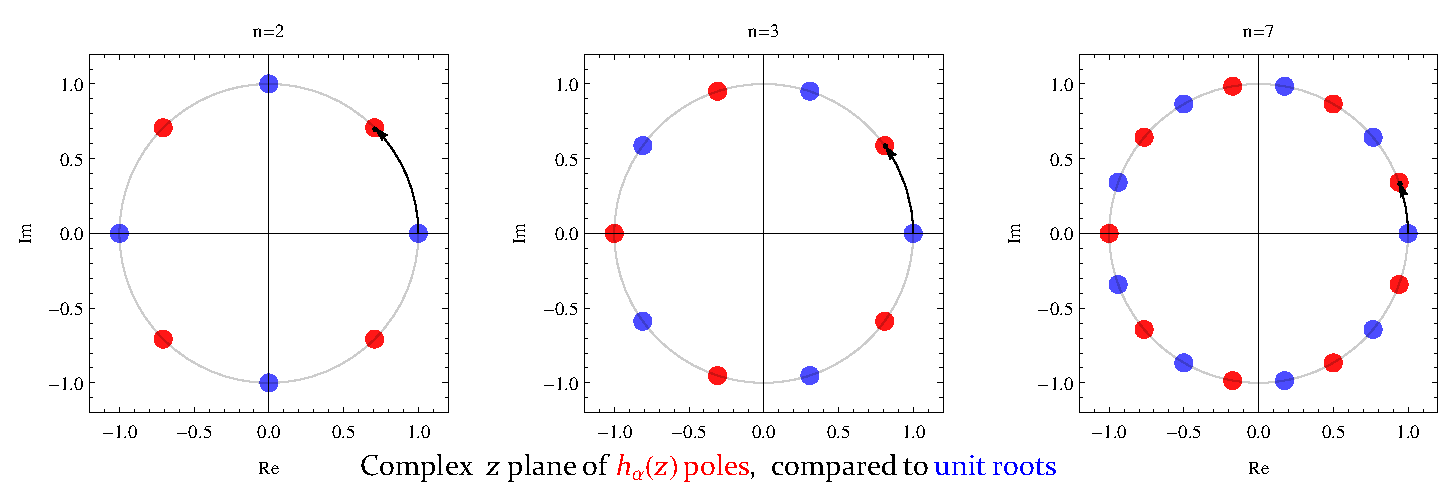
\includegraphics[width=\textwidth]{mathematica/wurzeln.pdf}
\caption{Unit roots in comparison to the poles of $h(z)/(2+n)=h(r)/2l$. Each pole occures two times, so the number of poles $|\{z_0\}|$ for given $n$ is $|\{z_0\}| = 2(n+2)$, while the number of unit roots $|\{x_0\}|$ is only $|\{x_0\}|=n+2$. The black arrow indicates the $e^{i\pi/(2+n)}$ rotation.} \label{fig:poles}
\end{figure}


\subsection{$\CA$ for $h(r)$ in $n$ dimensions}
%In this section, the exemplary calculations for $n=0$ from the previous section are repeated for general $n$.

Consider the holographic function in dimensionless coordinates $z=r L$ in $3+n$ dimensions:

\begin{align}
&h(z) = \frac 1{1+\left(\frac 1z\right)^{2+n}}
&h'(z) = \frac {(2+n) \left( \frac 1z \right)^{3+n}}
{\left( 1 + \left( \frac 1z \right)^{2+n} \right)^2}
\label{eq:hZn}
\end{align}

Calculating the Fourier transform of (\ref{eq:hZn}) can be done with Residue theorem, which requires knowledge of the poles, which are given when the demoninator of (\ref{eq:hZn}) equals 0. This problem can be reduced to determination of  the {\it roots of unity} (Einheitswurzeln):

\begin{equation}
z^{3+n} \left( 1 + \left( \frac 1z \right)^{2+n}\right)^2 = 0
\quad \Leftrightarrow \quad
1 = -z^{2+n}
\end{equation}

Given the $n$th root of unity, $x^n = 1$, and $-1 = e^{i\pi}$, the relation of the solution set $\{z_0\}$ and $\{x_0\}$ is given by $x_0 ~ e^{i\pi / (2+n)} = z_0$. Due to the power of 2 in the denominator, all poles of $h'(z)$ are doubled. See also figure \ref{fig:poles}.

Knowing the poles of the integrand, the integral can be performed by summing the residues.

\subsubsection{Results}
The results, done correctly, can be expressed with the Meijer G-function $\displaystyle
G_{p,q}^{\,m,n} \left( \left. \begin{matrix} a_1, \dots, a_p \\ b_1, \dots, b_q \end{matrix}\; \right| \; z \right)$. Table \ref{table:AforH} lists the results of the integral

\begin{equation}
\CA^{-2}(p) = 
\int \d r~(-1)^{n+1} \frac ip ~r^{n+1} \left(\Theta(-r) h'(-r) + \Theta(r) h'(r) \right) e^{-ipr}
\end{equation}

Constants like $\Omega_{n+2}/2$ as given in eq. (\ref{eq:FinalVpNdim}) are omitted.

\begin{table}[h]
\centering
\caption{Closed form expressions for $\CA^{-2}(p)$ for $h(r)$ in $n$ dimensions} \label{table:AforH}
$\begin{array}{cll}
\toprule
\mathbf{n} & 
\multicolumn{1}{c}{p \cdot \C A^{-2}(p)} \\
%\multicolumn{1}{c}{\mathbf{1}} \\
\midrule
\addlinespace
\mathbf{0} & 
  \begin{aligned}
-2 \sqrt{\pi } l G_{1,3}^{2,1}\left(\frac{l^2 p^2}{4}|
\begin{array}{c}
 -\frac{1}{2} \\
 \frac{1}{2},\frac{1}{2},0 \\
\end{array}
\right)
  \end{aligned} \\
\addlinespace


\midrule
\addlinespace
\mathbf{1} &
  \begin{aligned}
2 i \sqrt{\frac{3}{\pi }} l^2 G_{1,7}^{5,1}\left(\frac{l^6 p^6}{46656}|
\begin{array}{c}
 -\frac{1}{3} \\
 0,\frac{1}{6},\frac{1}{3},\frac{2}{3},\frac{2}{3},\frac{1}{2},\frac{5}{6} \\
\end{array}
\right)
  \end{aligned} \\
\addlinespace

\midrule
\addlinespace
\mathbf{2} &
  \begin{aligned}
-2 \sqrt{2 \pi } l^3 G_{1,5}^{3,1}\left(\frac{l^4 p^4}{256}|
\begin{array}{c}
 -\frac{3}{4} \\
 \frac{1}{4},\frac{1}{4},\frac{3}{4},0,\frac{1}{2} \\
\end{array}
\right)
  \end{aligned} \\
\addlinespace

\midrule
\addlinespace
\mathbf{3} &
  \begin{aligned}
2 i \sqrt{\frac{5}{\pi }} l^4 G_{1,11}^{7,1}\left(\frac{l^{10} p^{10}}{10000000000}|
\begin{array}{c}
 -\frac{2}{5} \\
 0,\frac{1}{10},\frac{1}{5},\frac{2}{5},\frac{3}{5},\frac{3}{5},\frac{4}{5},\frac{3}{10},\frac{1}{2},\frac{7}{10},\frac{9}{10} \\
\end{array}
\right)
  \end{aligned} \\
\addlinespace

\midrule
\addlinespace
\mathbf{4} &
  \begin{aligned}
-2 \sqrt{3 \pi } l^5 G_{1,7}^{4,1}\left(\frac{l^6 p^6}{46656}|
\begin{array}{c}
 -\frac{5}{6} \\
 \frac{1}{6},\frac{1}{6},\frac{1}{2},\frac{5}{6},0,\frac{1}{3},\frac{2}{3} \\
\end{array}
\right)
  \end{aligned} \\
\addlinespace

\midrule
\addlinespace
\mathbf{5} &
  \begin{aligned}
2 i \sqrt{\frac{7}{\pi }} l^6 G_{1,15}^{9,1}\left(\frac{l^{14} p^{14}}{11112006825558016}|
\begin{array}{c}
 -\frac{3}{7} \\
 0,\frac{1}{14},\frac{1}{7},\frac{2}{7},\frac{3}{7},\frac{4}{7},\frac{4}{7},\frac{5}{7},\frac{6}{7},\frac{3}{14},\frac{5}{14},\frac{1}{2},\frac{9}{14},\frac{11}{14},\frac{13}{14} \\
\end{array}
\right)
  \end{aligned} \\
\addlinespace


\bottomrule
\end{array}$
\end{table}


\subsection{$\CA$ for $h_\alpha(r)$ in $n$ dimensions}
When studying the self-regular profile in dimensionless coordinates $z=rL$ in $3+n$ dimensions:

\begin{align}
&h_\alpha(z) = \frac{1}{\left(1+\left(\frac 1z\right)^\alpha / 2\right)^{\frac {3+n}{\alpha}}}
%
&h'_\alpha(z) = \frac{ \frac {3+n}{2} \left( \frac 1z \right)^{\alpha+1}} {\left(1+\left(\frac 1z\right)^\alpha / 2\right)^{\frac {3+n}{\alpha} + 1}}
\end{align}

It is hard to find a closed form expression for the Fourier transform $\C F\{ h'_\alpha(z) \}$ even for $n=0$, but in principle it should be possible, since the roots should be clearly determinable.





\end{document}